\hypertarget{dqagp_8f}{
\section{/home/mgh/LanlGeoMag/libLanlGeoMag/dqagp.f File Reference}
\label{dqagp_8f}\index{/home/mgh/LanlGeoMag/libLanlGeoMag/dqagp.f@{/home/mgh/LanlGeoMag/libLanlGeoMag/dqagp.f}}
}
\subsection*{Functions}
\begin{CompactItemize}
\item 
subroutine \hyperlink{dqagp_8f_3809d8d2a43b03d1f3c0f7833c0d82c8}{DQAGP} (F, A, B, NPTS2, POINTS, EPSABS, EPSREL, RESULT, ABSERR, NEVAL, IER, LENIW, LENW, LAST, IWORK, WORK)
\end{CompactItemize}


\subsection{Function Documentation}
\hypertarget{dqagp_8f_3809d8d2a43b03d1f3c0f7833c0d82c8}{
\index{dqagp.f@{dqagp.f}!DQAGP@{DQAGP}}
\index{DQAGP@{DQAGP}!dqagp.f@{dqagp.f}}
\subsubsection[{DQAGP}]{\setlength{\rightskip}{0pt plus 5cm}subroutine DQAGP (DOUBLE PRECISION,external {\em F}, \/  DOUBLE PRECISION {\em A}, \/  DOUBLE PRECISION {\em B}, \/  INTEGER {\em NPTS2}, \/  DOUBLE PRECISION,dimension($\ast$),dimension {\em POINTS}, \/  DOUBLE PRECISION {\em EPSABS}, \/  DOUBLE PRECISION {\em EPSREL}, \/  DOUBLE PRECISION {\em RESULT}, \/  DOUBLE PRECISION {\em ABSERR}, \/  INTEGER {\em NEVAL}, \/  INTEGER {\em IER}, \/  INTEGER {\em LENIW}, \/  INTEGER {\em LENW}, \/  INTEGER {\em LAST}, \/  INTEGER,dimension($\ast$),dimension {\em IWORK}, \/  DOUBLE PRECISION,dimension($\ast$),dimension {\em WORK})}}
\label{dqagp_8f_3809d8d2a43b03d1f3c0f7833c0d82c8}




Definition at line 2 of file dqagp.f.

Here is the call graph for this function:\nopagebreak
\begin{figure}[H]
\begin{center}
\leavevmode
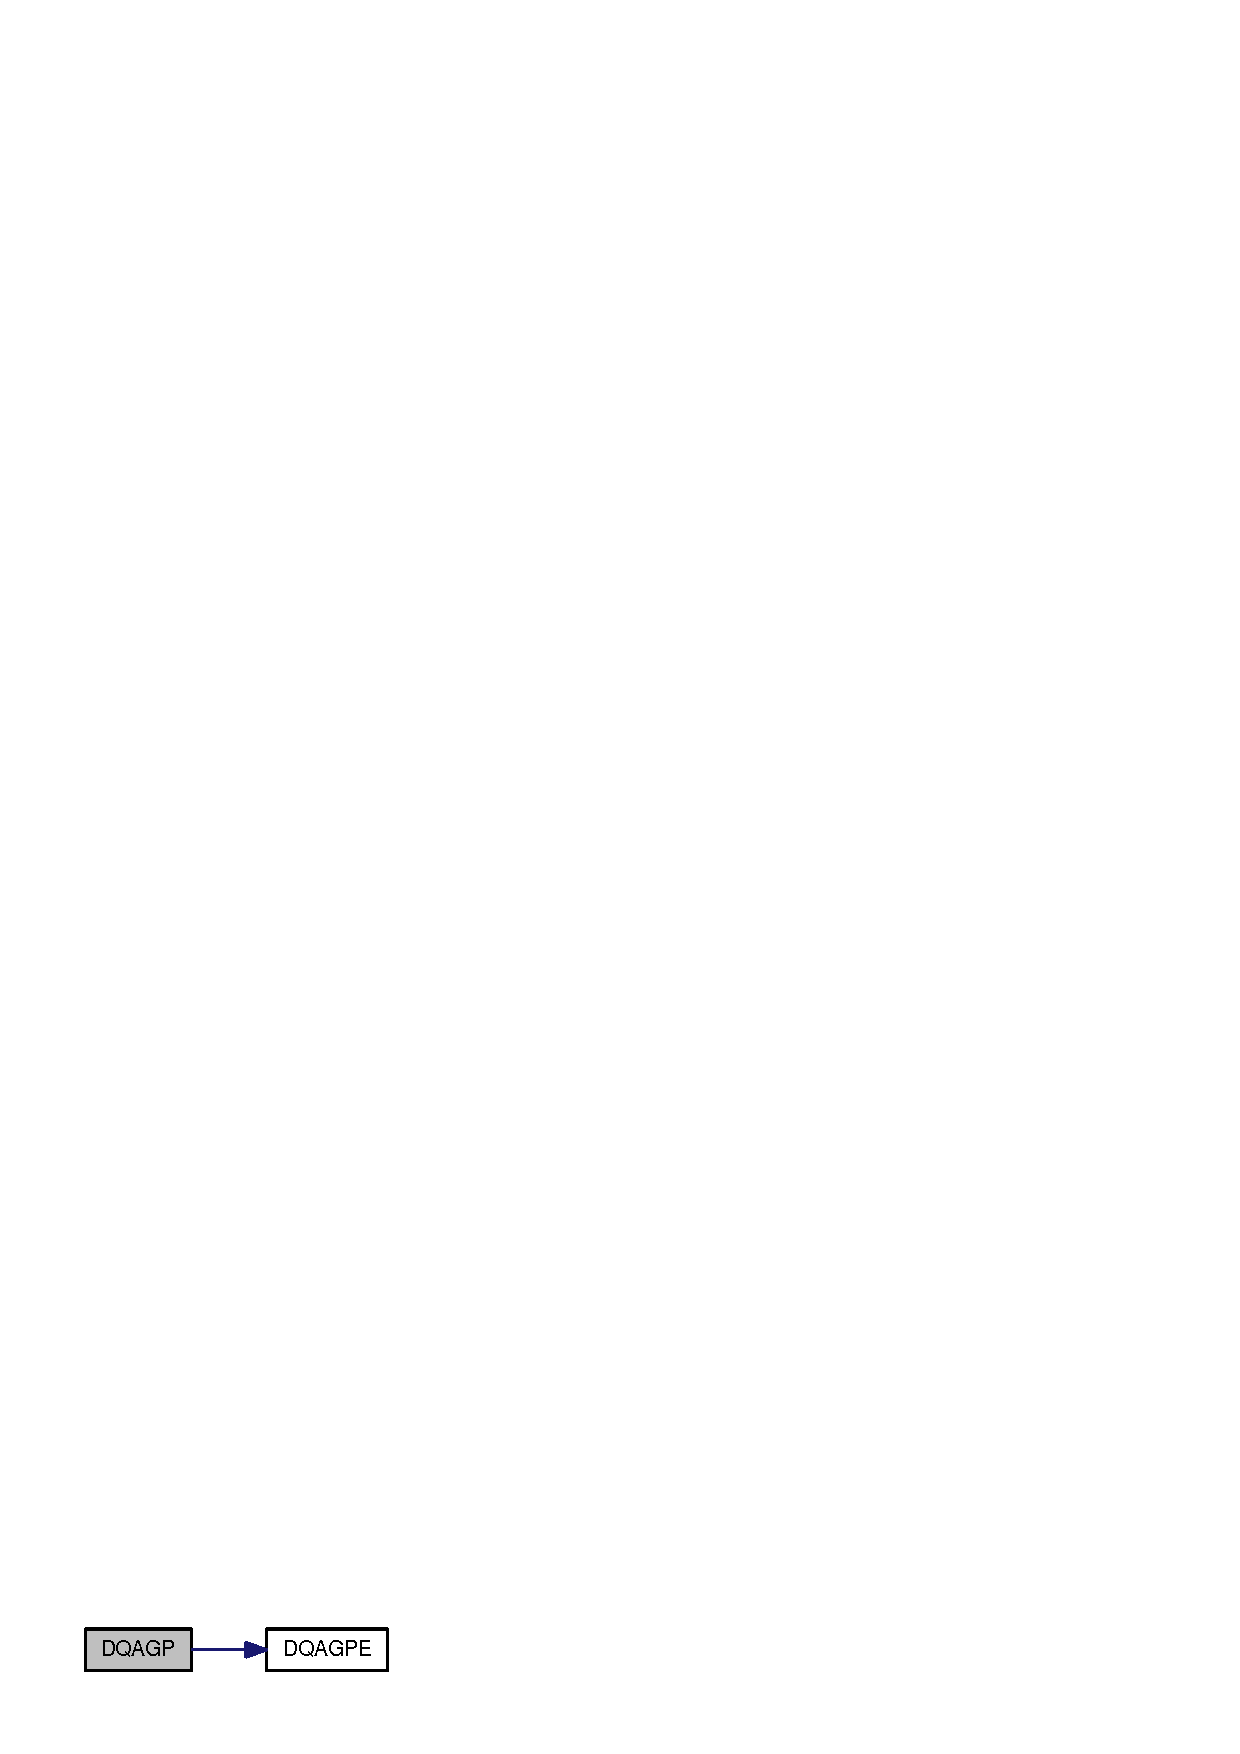
\includegraphics[width=95pt]{dqagp_8f_3809d8d2a43b03d1f3c0f7833c0d82c8_cgraph}
\end{center}
\end{figure}
